\documentclass[letterpaper,10pt]{article}

\usepackage{tabularx} % extra features for tabular environment
\usepackage{amsmath}  % improve math presentation
\usepackage{graphicx} % takes care of graphic including machinery
\usepackage[margin=1in,letterpaper]{geometry} % decreases margins
\usepackage{cite} % takes care of citations
\usepackage[final]{hyperref} % adds hyper links inside the generated pdf file
\usepackage{ctex}
\usepackage{titlesec}
%\usepackage{CJKutf8, CJK}
\usepackage{makecell}                 % 三线表-竖线
\usepackage{booktabs}                 % 三线表-短细横线
% \usepackage{natbib}
\usepackage{graphicx}				  % 表格单元格逆时针
\usepackage{multirow}				  % 合并单元格
\usepackage{array}
\usepackage{amssymb}				  % 勾
\usepackage{amsmath}
\usepackage{longtable}                % 导入 longtable 宏包,表格自动换行
\usepackage{caption}
\usepackage{subcaption}               % 设置子图
\usepackage{color}					  % 文本颜色包
\usepackage{xcolor}
\usepackage{bbm}					  % 输入指示函数
\usepackage{tablefootnote}			  % 表格注释
\usepackage{pythonhighlight}
\usepackage{fancyhdr}
\usepackage{lastpage}
\pagestyle{fancy}
\fancyhf{}
\fancyhead{}
\fancyfoot{}
\fancyhead[R]{\small Page \thepage\ of \pageref*{LastPage}}
\fancyhead[L]{\small Report}

\usepackage{listings}                 % 导入代码块
\usepackage{xcolor}
\lstset{
	numbers=left, 
	tabsize=1,
	columns=flexible, 
	numberstyle=  \small, 
	keywordstyle= \color{ blue!70},
	commentstyle= \color{red!50!green!50!blue!50}, 
	frame=shadowbox, % 阴影效果
	rulesepcolor= \color{ red!20!green!20!blue!20} ,
	escapeinside=``, % 英文分号中可写入中文
	xleftmargin=2em,
	xrightmargin=2em, 
	aboveskip=1em,
} 

\hypersetup{
	colorlinks=true,       % false: boxed links; true: colored links
	linkcolor=blue,        % color of internal links
	citecolor=blue,        % color of links to bibliography
	filecolor=magenta,     % color of file links
	urlcolor=blue         
}
%++++++++++++++++++++++++++++++++++++++++
\titleformat{\section}{\Large\bfseries\songti}{\thesection}{1em}{}
\titleformat{\subsection}{\large\bfseries\songti}{\thesubsection}{1em}{}
\titleformat{\subsubsection}{\normalsize\bfseries\songti}{\thesubsubsection}{1em}{}
\titleformat{\paragraph}{\small\bfseries\songti}{\paragraph}{1em}{}
\titleformat{\subparagraph}{\footnotesize\bfseries\songti}{\subparagraph}{1em}{}

\begin{document}
	
	
	\title{\songti \zihao{4}7月17日-7月23日工作汇报}
	\author{\textrm{Ku Jui}}
	\date{\textrm{July 2023}}
	\maketitle
	
	\renewcommand{\figurename}{Figure} % 可以重新定义abstract,因为ctex会覆盖thebibliography
	% 	\begin{abstract}
		%		In this experiment we studied a very important physical effect by measuring the
		%		dependence of a quantity $V$ of the quantity $X$ for two different sample
		%		temperatures.  Our experimental measurements confirmed the quadratic dependence
		%		$V = kX^2$ predicted by Someone's first law. The value of the mystery parameter
		%		$k = 15.4\pm 0.5$~s was extracted from the fit. This value is
		%		not consistent with the theoretically predicted $k_{theory}=17.34$~s. We attribute %this
		%		discrepancy to low efficiency of our $V$-detector.
		%	\end{abstract}
	\renewcommand{\contentsname}{Contents}
	\renewcommand{\tablename}{Table}
	\tableofcontents  % 自动生成目录
	
	\part{Pre-Knowledge}
	
	\section{Application scenarios}
	
	在硬件条件不变的情况下,给定降质图像或恶劣天气下拍摄的图像,研究生成高质量、高分辨率、无噪声图像的超分辨率等增强方法,在实际应用中非常有意义。基于软件技术的图像复原增强技术得到了广泛研究,其通过引入外部信息、加入先验、基于大数据集进行学习等方式,将输入的低分辨率图像或带噪图的高频细节复原,产生接近降质前理想高分辨率的无噪图。低质图像重建在安防监控、遥感成像、医学影响成像、消费电子以及室外监控等领域得到广泛应用。
	
		\subsection{安防监控领域}
		
		视频监控设备作为安防系统的输人终端,提供了最基础的案件复原、实时监控的素材,在案情预防、分析和侦破等方面发挥着非常重要的作用。然而,实际场景的监控视频质量却往往与侦查机关的案件侦察办理需求之间存在差距。一方面,实地部署的摄像头硬件的成像条件有限;另一方面,为了控制存储空间和传输成本,监控视频往往使用较低的码率进行压缩存储,导致视频中很多细节的丢失。许多对破案有意义的视频信息,在压缩存储和传输的过程中遭到丢失。这时利用低质图像、视频复原技术,能够将低质量的监控视频增强为高质量的目标视烦,便于进一步进行人工分析或后续的自动识别;也可通过对感兴趣区域进行跟踪和放大,对人脸、行人或车牌等进行识别。
		
		\subsection{遥感成像领域}
		
		卫星遥感具有持续时间长、覆盖面积广、实时性强、不受地城限制等优点,被广泛应用于环境监测、灾害预警与救授、资源开发、地域变化分析等领域。然而,在使用卫星和无人机进行遥感图像采集的过程中,受大气扰动、光照条件、成像系统的物理极限以及卫星、无人机等平台震颤等因素彤响,釆集得到的图像包含各类降质问题,增加了后续处理的难度,制约了遥感图像的应用。低质图像重建技术能够对遥感图像进行分辨率增强,移除图像中的降质因素,从而提升遥感图像的质量,便于后续分析与处理。
		
		\subsection{医学影像成像领域}
		
		近几十年来,医学影像技术取得了迅速的发展。X射线、CT、超声、核磁共振等技术在临床上得到了广泛应用。其中,核磁共振的成像原理是利用共振效应,从人体中获取电磁信号,并根据这些信号绘制出人体信息。但是,核磁共振图像的成像分辨率受到许多因素的制约,比如信噪比、患者进行图像扫描时的舒适程度、硬件条件、扫描时间等。因此,扫描得到的图像可能出现分辨率不足的问题。同时,仅对人体的一个断层进行扫描,并不能获得所有信息。通过低质医学图像的复原重建技术,可以根据采集到的多张低分辨率扫描图像重建出高分辨率图像,从而恢复出完整的组织细节,为医生提供更好的诊断依据。如Fig. \ref{fig: Super resolution reconstruction}所示,超分辨率重建填补了核磁共振扫描图像中的细节。
	
	    \begin{figure}[htbp] 
		% read manual to see what [ht] means and for other possible options
		\centering 
		
		\begin{subfigure}{0.15\textwidth}
			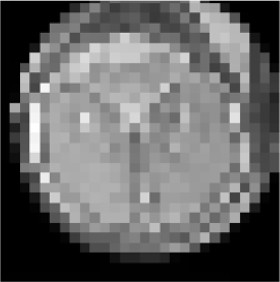
\includegraphics[width=\linewidth]{picture/LR}
			\captionsetup{font=scriptsize}
			\label{fig:LR input}
		\end{subfigure}
		\begin{subfigure}{0.15\textwidth}
			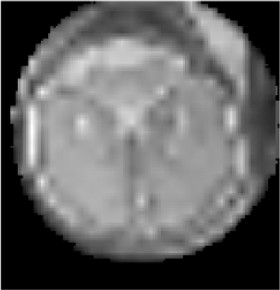
\includegraphics[width=\linewidth]{picture/linear}
			\captionsetup{font=scriptsize}
			\label{fig: Linear}
		\end{subfigure}
		\begin{subfigure}{0.15\textwidth}
			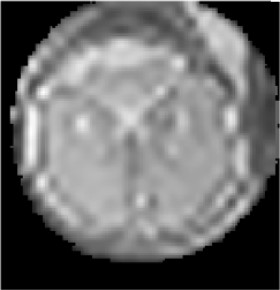
\includegraphics[width=\linewidth]{picture/B-spline}
			\captionsetup{font=scriptsize}
			\label{fig: B-spline}	
		\end{subfigure}
		\begin{subfigure}{0.15\textwidth}
			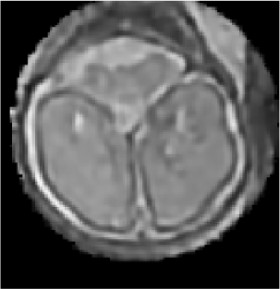
\includegraphics[width=\linewidth]{picture/3D-MRI-CNN}
			\captionsetup{font=scriptsize}
			\label{fig: 3D MRI CNN}
		\end{subfigure}
		\begin{subfigure}{0.15\textwidth}
			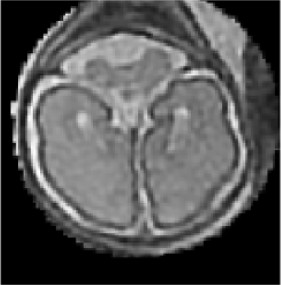
\includegraphics[width=\linewidth]{picture/GT-HR}
			\captionsetup{font=scriptsize}
			\label{fig: GT HR}
		\end{subfigure}
		\captionsetup{font=scriptsize}
		\caption{
			\label{fig: Super resolution reconstruction}
			超分辨率重建在核磁共振成像中的应用 \cite{McDonagh_2017}
		}
	    \end{figure}
	
		\subsection{消费电子领域}
		
		近十年来,新兴多媒体应用快速发展,低质图像、视频重建技术在消费电子领城的应用呈现井喷之势,例如老照片的划痕和折痕去除、污渍或空白区域填充、视频中遮挡物的移除、黑白老照片的彩色化、数字照相机内的自动光照调整和噪声去除、相机内针对拍摄时延以及抖动的去模糊复原等。随着高清电视(high drtniion tolerision, HDTV)的大规模推广使用以及虚拟现实技术实用化的发展,一方面,现有的视顿播放片源仅有少部分能生满足高清电视的播放要求,另一方面,现有的带宽资源很难在分辨率上满足沉浸式体验的需求。因此,一个有效的解决途径是在客户端通过低质视频重建技术复原解码出高清图像,或根据多个视角的低分辨率图像,融合得到高清图像,并移除其他降质因素的影响。
	
		\subsection{室外监控领域}
		
		随着智慧城市的不断发展,室外监控逐渐覆盖公共生活的方方面面。然而,由于室外拍摄环境较为复杂,监控视频会受到各种各样降质因素的影响,比如雨天拍摄的视频中雨点对背景的遮挡、大雾天气下能见度的降低、低光照环境下大量物体信号的丢失、雨雾环境下大量物体细节的丢失等。这些因素对后续的人工分析和计算机视觉应用造成了障得。而使用低质图像、视频重建技术对这些因素进行移除,能够提升图像、视频的能见度,增强高频细节,便于后续处理与分析。如Fig. \ref{fig: Rainy image marks}所示,对雨天图像进行雨痕去除,能够提升图像的视觉质量,并使图像识别结果变得正确。
	
		\begin{figure}[htbp] 
		% read manual to see what [ht] means and for other possible options
		\centering 
		% 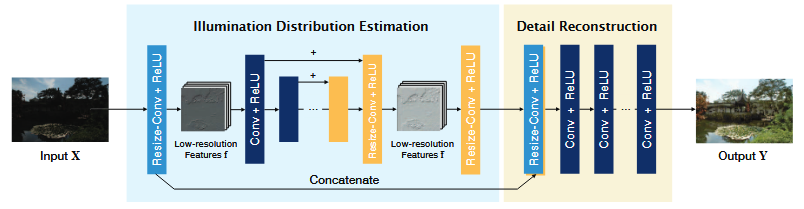
\includegraphics[width=0.8\columnwidth]{GLADNet}
		
		\begin{subfigure}{0.4\textwidth}
			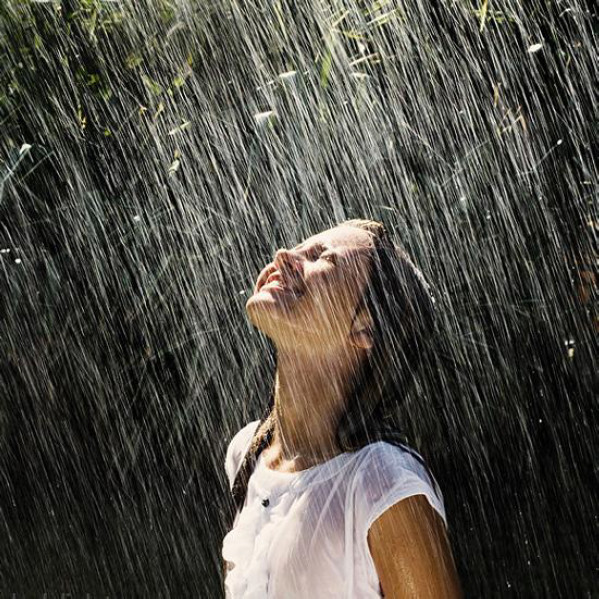
\includegraphics[width=\linewidth]{picture/rain}
			\captionsetup{font=scriptsize}
			\label{fig:rain}
		\end{subfigure}
		\begin{subfigure}{0.4\textwidth}
			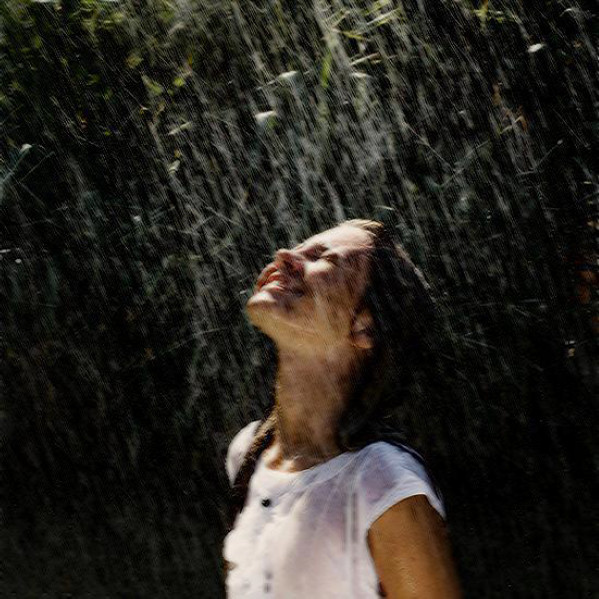
\includegraphics[width=\linewidth]{picture/people}
			\captionsetup{font=scriptsize}
			\label{fig:people}
		\end{subfigure}\\
		\begin{subfigure}{0.4\textwidth}
			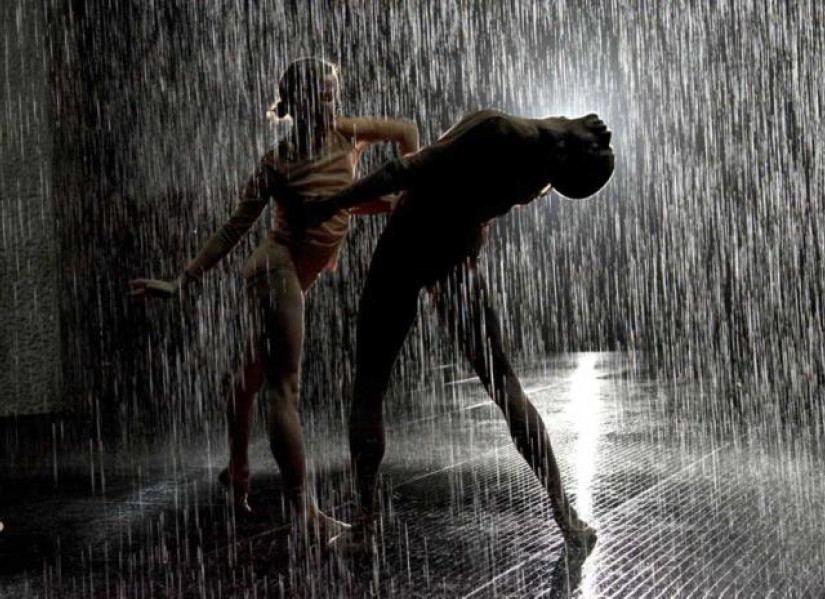
\includegraphics[width=\linewidth]{picture/rain1}
			\captionsetup{font=scriptsize}
			\caption{有雨图像输入}
			\label{fig:rain1}	
		\end{subfigure}
		\begin{subfigure}{0.4\textwidth}
			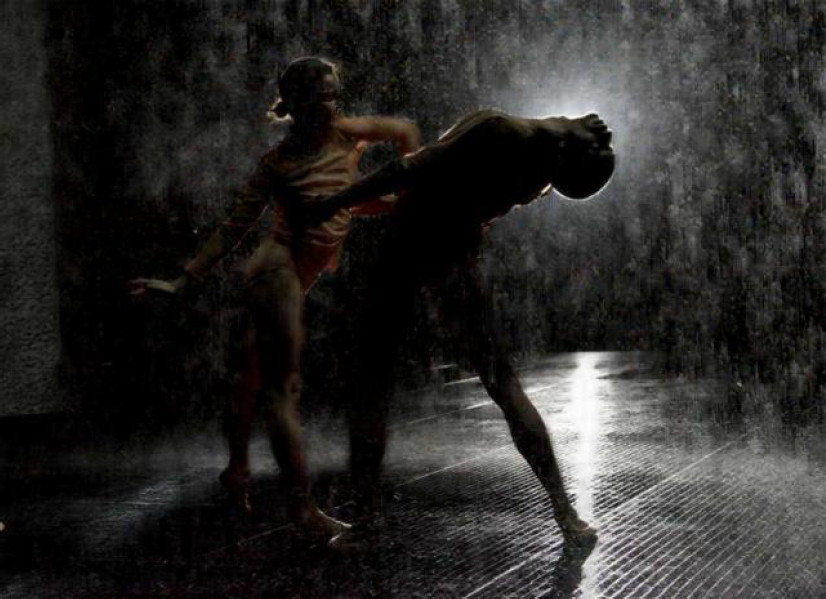
\includegraphics[width=\linewidth]{picture/people1}
			\captionsetup{font=scriptsize}
			\caption{去雨结果}
			\label{fig:people1}
		\end{subfigure}
		\captionsetup{font=scriptsize}
		\caption{
			\label{fig: Rainy image marks}
			雨天图像雨痕去除结果 \cite{yang2017deep}
		}
	    \end{figure}
	

%	\begin{itemize}
%		\item {}
%			Tranformer相较于CNN结构,缺少一定的平移不变性和局部感知性,因此在数据量不充分时,很难达到同等的效果。具体表现为使用中等规模的ImageNet训练的Tranformer会比ResNet在精度上低几个百分点。
%		\item {}
%			当有大量的训练样本时,结果则会发生改变。使用大规模数据集进行预训练后,再使用迁移学习的方式应用到其他数据集上,可以达到或超越SOTA水平。
%	\end{itemize}
%	
%
%	\begin{itemize}
%		\item {}
%			BiT算法\cite{kolesnikov2020big}:使用大规模数据集 JFT-300M 对 \texttt{ResNet} 结构进行预训练,其中,作者发现模型越大,预训练效果越好,最终指标最高的为4倍宽、152层深的$\texttt{ResNet}152\times 4$。
%		\item {}
%			Noisy Student 算法\cite{xie2020self}:使用知识蒸馏的技术,基于 \texttt{EfficientNet} 结构,利用未标签数据,提高训练精度。
%	\end{itemize}	

	\section{Traditional Low-Light Image Enhancement Method}
	
	根据传统方法的图像低光照增强算法通常利用单张图像自身的性质进行图像增强。根据基于的先验不同,可以分为基于直方图的方法、基于图像反相的方法和基于Retinex模型的方法3类。
	
	
		\subsection{基于直方图的方法}
		
		基于直方图的方法主要考虑直方图均衡化,通过对直方图\footnote{直方图统计图像每个灰度级的出现频率,其横坐标表示灰度级,纵坐标表示像素值为该灰度级下像素的频率。}的分布进行约束,改善图像的亮度分布。直方图描述了图像灰度级\footnote{图像灰度(image grayscale):把白色与黑色之间按对数关系分为若干等级,称为灰度。灰度分为256阶。用灰度表示的图像称作灰度图。}的分布情况,显示了图像的灰度范围和每个灰度级的出现频率。摄影师也常利用直方图判断整幅图像的明暗程度、对比度等图像特征,以便完成相应的后期处理。
		
        \begin{figure}[htbp]
			% read manual to see what [ht] means and for other possible options
			\centering 
			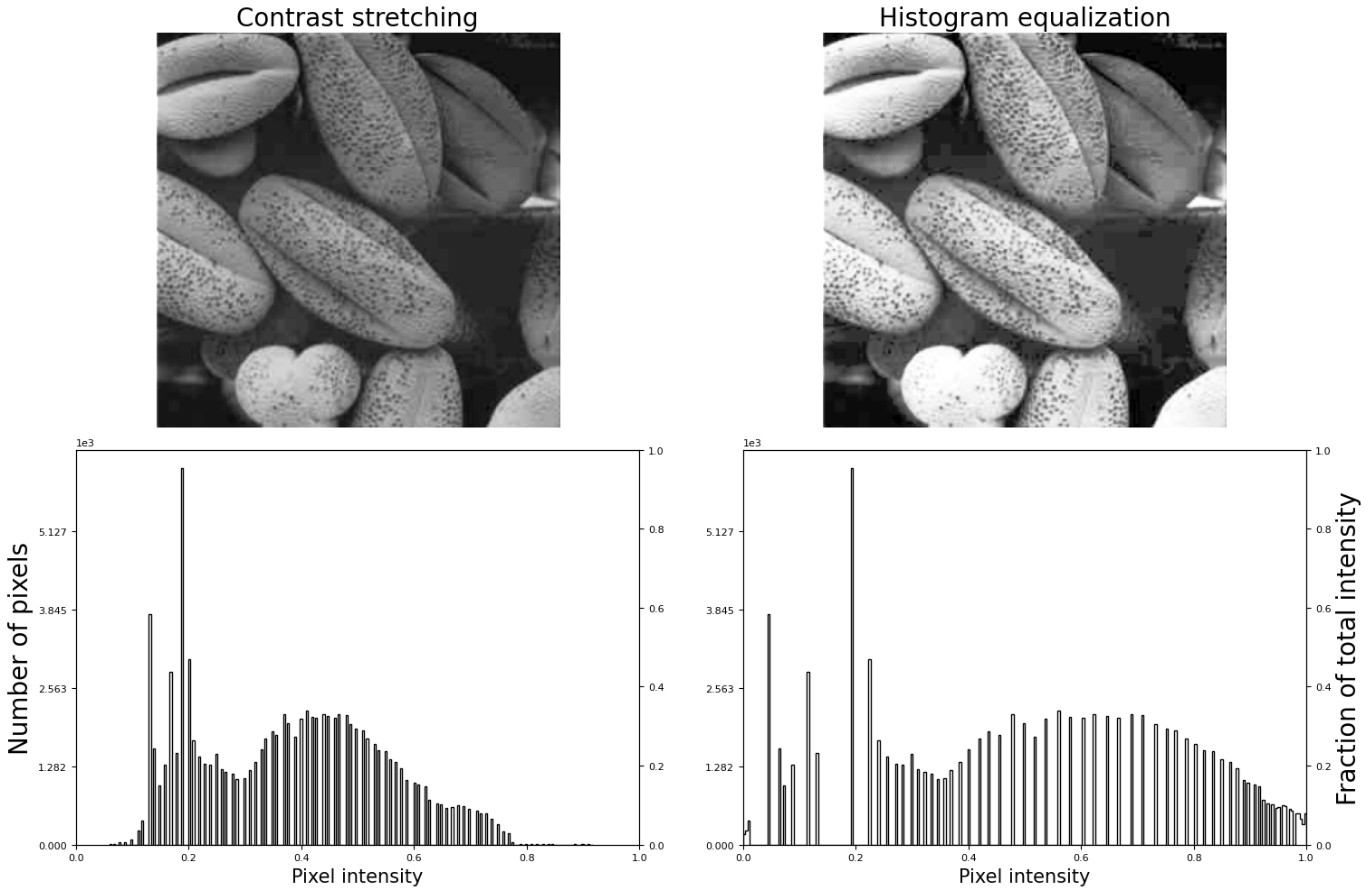
\includegraphics[width=\columnwidth]{picture/Histogram equalization}
			%\captionsetup{font=scriptsize}
			\caption{
				\label{fig: Histogram equalization} 
				直方图均衡化示意图
			}
		\end{figure}
		
		如Fig. \ref{fig: Histogram equalization}所示,直方图均衡化重新调整图像的直方图分布,一方面增加了图像的全局对比度,另一方面使得亮度在整个图像的分布更加均匀。考虑一张包含L个灰度级的图像,其直方图可以表示为:
		
		\begin{equation}
			\begin{aligned}
				P(r_k) = \frac{n_k}{n}, k=0, 1, 2, \cdots, L-1
			\end{aligned}
			\label{eq: Histogram}
		\end{equation}
		
		其中, $r_k$ 表示第 $k$ 级灰度值,$n_k$表示图像中第 $k$ 级灰度值所对应的像素个数,$n$ 表示图像中的所有像素总数。显然,有 $\sum_{k} P(r_k)=1$。直方图均衡化是指存在一个变换函数 $s=T(r), 0 \leqslant r \leqslant 1$,能够将灰度级 $r$ 转化为灰度级 $s$。$T(r)$满足以下两个条件: 首先,$T(r)$ 在区间 $[0, 1]$ 上为单射函数且单调递增; 其次, $T(r) \in [0, 1]$ 。$T(r)$ 是单射函数保证了直方图均衡化存在反变换,而其单调递增的性质保证了变化后的图像与原图像之间存在保序性,以防变换后图像发生黑白颠倒。
		
		这样,一幅图像的灰度即视为 $[0,1]$ 上的随机变量,用 $p_r(r)$ 和 $p_s(s)$ 表示随机变量 $r$ 与 $s$的概率密度函数,那么,直方图均衡化即将 $T(r)$ 表示如下: $$s = T(r) = \int_{0}^{r} p_r(w) \mathrm{d}w$$ 可以证得,通过 $T(r)$ 的转化,有 $p_s(s) = 1$ ,即转换后的像素值在 $[0, 1]$ 上均匀分布。这时基于直方图变换的保序性,有 $$\int_{0}^{n} p_r(r) \mathrm{d}r = \int_{0}^{T(n)} p_s(s) \mathrm{d}s$$ 从而有: $$\frac{\mathrm{d}s}{\mathrm{d}r} = \frac{\mathrm{d}T(r)}{\mathrm{d}r} = p_r(r)$$ 代入上式,可得: $$p_s(s) = 1$$ 
		
		直方图均衡化的方法非常快速有效,并且是一个可逆操作,但缺点在于其不加选择地处理数据,可能增加背景噪声的对比度,同时降低有用的图像内容的对比度,导致视觉效果欠佳。此外,该方法也无法适用于复杂多变的低光照场景。
		
		\subsection{基于图像反相的方法}
		
		\begin{figure}[htbp] 
			% read manual to see what [ht] means and for other possible options
			\centering 
			% 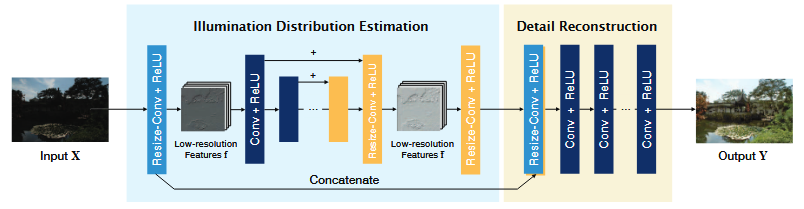
\includegraphics[width=0.8\columnwidth]{GLADNet}
			
			\begin{subfigure}{0.18\textwidth}
				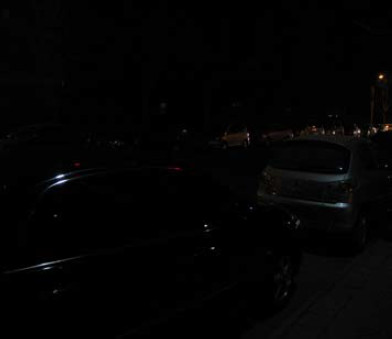
\includegraphics[width=\linewidth]{picture/LL input}
				\captionsetup{font=scriptsize}
				\label{fig: LL input}
			\end{subfigure}
			\begin{subfigure}{0.18\textwidth}
				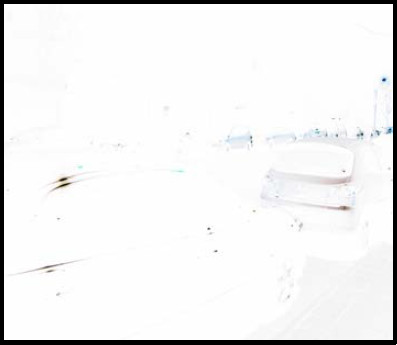
\includegraphics[width=\linewidth]{picture/Inversed}
				\captionsetup{font=scriptsize}
				\label{fig: Inversed}
			\end{subfigure}
			\begin{subfigure}{0.18\textwidth}
				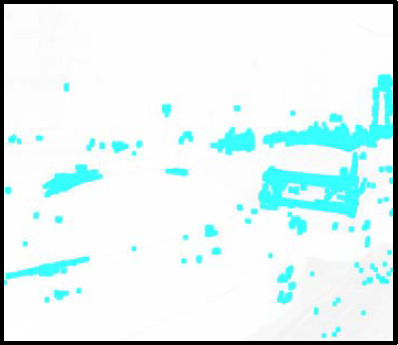
\includegraphics[width=\linewidth]{picture/marked image}
				\captionsetup{font=scriptsize}
				\label{fig: marked image}	
			\end{subfigure}
			\begin{subfigure}{0.18\textwidth}
				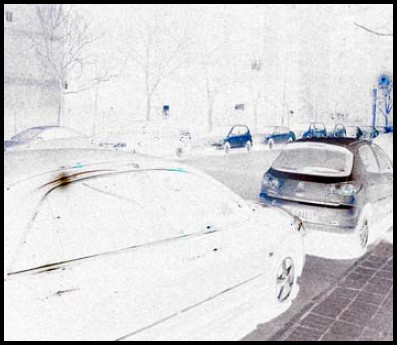
\includegraphics[width=\linewidth]{picture/de-haze}
				\captionsetup{font=scriptsize}
				\label{fig: de-haze}
			\end{subfigure}
			\begin{subfigure}{0.18\textwidth}
				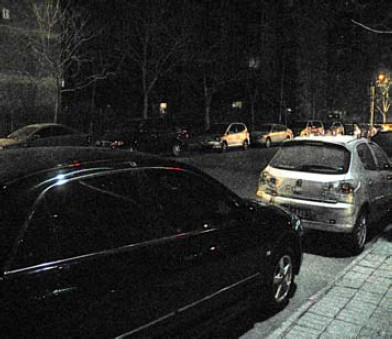
\includegraphics[width=\linewidth]{picture/Final output}
				\captionsetup{font=scriptsize}
				\label{fig: Final output}
			\end{subfigure}
			\captionsetup{font=scriptsize}
			\caption{
				\label{fig: Image Inverse}
				(a) low lighting video input I. (b) inverted result R from input I. (c) marked image: pixels with low intensity in at least one
				color (RGB) channel are in green. (d) de-haze output J using equation (7). (e) final output E after inverting image J.
			}
		\end{figure}
		
		基于图像反相的方法\cite{10.1145/1836845.1836920}利用低光照图像的反相\footnote{图像反相 (Image reverse phase) 就是图像的颜色色相反转。以前照相机的底片就是打印后的照片的反相。比如黑变白,蓝变黄、红变绿。对灰度级范围为 $[0 , L-1]$ 的一幅图像进行反转的操作为:$s = L - 1 - r$ 其中$r$和$s$分别代表处理前后的像素值。使用这种方式反转一幅图像的灰度级,可得到等效的照片底片。这种类型的处理特别适用于增强嵌入在一幅图像的暗区域中的白色和灰色细节,特别是当黑色面积在尺寸上占主导地位时}与有雾图像的相似性,通过对低光照图像反相进行去雾后再次进行反相,得到最终的低光照增强效果。在图像反相中,对于动态范围为 $[ 0, 255]$ 的图像,其反相图像 $\mathbf{R}$ 为: 
		
		\begin{equation}
			\begin{aligned}
				\mathbf{R}^c (x) = 255 - \mathbf{I}^c(x)
			\end{aligned}
			\label{eq: Image Reverse}
		\end{equation}
		
		其中,$c$ 为 \textbf{RGB} 颜色通道。大多数有雾图像符合暗通道先验,其特点是对于背景及天空等区域,\textbf{RGB} 3个通道的像素值都很高,而其他区域至少有一个通道的像素值较低,作者发现低光照图像的反相也具有同样特点。如Fig. \ref{fig: Image Inverse}
		
		基于图像反相的方法虽然运算速度很快,但需要基于低光照图像反相与有雾图像相似这一前提,而改前提始终是统计意义上的,无法得出二者之间更本质的联系,因而限制了这一方法的继续发展。由于没有考虑低光照图像的结构信息,因此该类方法还常常导致增强结构出现明显的黑边。
		
		\subsection{Retinex模型}
		
		
	
	\section{Modern Low-Light Image Enhancement Method}
		
		\subsection{Deep Learning for Low-Light Image Enhancement}
	
		\subsection{Low-Light Image Enhancement based on the Retinex Model}
		
	
	\section{Image Super Resolution}
	
		\subsection{Image Super-resolution Problem Definition}
		
		\subsection{Super-resolution Convolutional Neural Network Reconstruction}
		
		\subsection{Very Deep Super Resolution, VDSR}
		
		\subsection{Fast Super-resolution Reconstruction}
		
		\subsection{Super-resolution Generative Adversarial Networks}
		
	
	\section{Follow-up specific work}
	
		\subsection{方向一}
		
		Retinex-Net 在测试图像时会造成颜色失真,这可能是由于网络无法同时兼顾如亮度\footnote{图像的亮度是指图像像素的大小,像素值越大,图像在该像素点越明亮,否则越暗。对于灰度图像来说,每个像素点只有 1 个分量,且在 $0 \sim 255$ 之间,0 表示黑色,最暗,255 表示白色,最亮。}、对比度\footnote{图像的对比度是指一幅图像中明暗区域最亮的白和最暗的黑之间不同亮度层级的测量,即一幅图像灰度反差的大小,通俗一点来说就是最大亮度与最小亮度之比,如 Michelson 对比度被定义为:$$C_M = \frac{I_{max} - I_{min}}{I_{max} + I_{min}}$$},伪影\footnote{伪影(Artifacts),是指原本被拍摄物体并不存在而在图像上却出现各种形态的影像。在图像处理后,尤其在合成图片中,表现为不自然的、能让人看出是人为处理过的痕迹、区域、瑕疵等。成像系统做图片重建时会产生一些伪影问题,产生这种现象的原因主要是由于图像处理的不精确或者信息缺失。部分现象展示如Fig. \ref{fig: Ringing Artifacts}。
		
		}等各种因素造成的。同时它只局限于对低光照图像的处理并没有扩展到视频等领域。
		(2018年)模型MBLLEN\cite{Lv2018MBLLEN}适用性相对于Retinex-Net模型适用性更加广阔,对低光视频改善也有不错的效果,其提出了多分支低光增强网络,它可以兼顾如亮度、对比度,伪影等,其核心思想是提取不同层次的丰富特征,这样可以通过子网进行增强,最后通过多分支融合输出图像。
		
		\begin{figure}[htbp]
			% read manual to see what [ht] means and for other possible options
			\centering 
			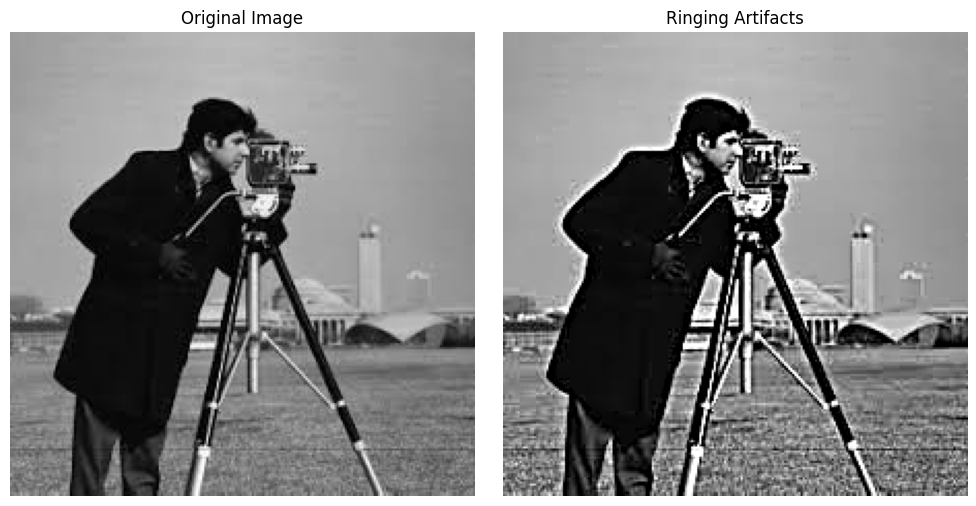
\includegraphics[width=0.5\columnwidth]{picture/Artifacts}
			%\captionsetup{font=scriptsize}
			\caption{
				\label{fig: Ringing Artifacts} 
				边界伪影。
			}
		\end{figure}
		
		\begin{itemize}
			\item{}
			单分支或简单神经网络不能同时进行亮度、对比度增强和伪影去除、降噪等多功能需求;
			\item{}
			由于图像和视频承载着丰富而详细的真实的场景信息,真实的系统严重依赖于输入它们的质量。特别地,它们可能在高质量输入数据的情况下表示良好,但在其他情况下表现不佳。一种典型的情况是使用在照明不良的环境中捕获的图像。当相机在捕获期间不能接收足够的光时,将在暗区域中存在信息丢失和意外噪声。
		\end{itemize}
	
		因此可以\textbf {\color{red}{仔细研究其特征提取模块(FEM)}加以改进用于图像融合的特征提取当中,其融合方法也可以改进,用于其他领域作为最后的图像重建阶段。多分支的思想也可以作为一个模块用于其他方法中。}
		
		\paragraph{Plan}
		
		\begin{itemize}
			\item[ 1)]
			复现MBLLEN源码,研究其特征提取模块(FEM)。数据集部分可以使用MBLLEN论文中提供的数据集。
			\item[ 2)]
			理解图像特征融合\footnote{图像特征融合(Image feature fusion)是指将图像中提取出的特征进行组合。它的目的是把从图像中提取的特征,合并成一个比输入特征更具有判别能力的特征。特征融合方法是模式识别领域的一种重要的方法,计算机视觉领域的图像识别问题作为一种特殊的模式分类问题,仍然存在很多的挑战,特征融合方法能够综合利用多种图像特征,实现多特征的优势互补,获得更加鲁棒和准确性的识别结果}的方式,以及了解如何实现图像特征融合。
		\end{itemize}
	
		\subsection{方向二}
	
		
	
	
%%%%%%%%%%%%%%%%%%%%%%%%%%%%%%%%%%%%%%%%%%%%%%%%%%%%%%%%%%%%%%%%%%%%%%%%%%%%%%%%%%%%%%%%%%%%%%%%%%%%
%%%%%%%%%%%%%%%%%%%%%%%%%%%%%%%%%%%%%%%%%%%%%%%%%%%%%%%%%%%%%%%%%%%%%%%%%%%%%%%%%%%%%%%%%%%%%%%%%%%%
%%                                                                                                %% 
%%								          Paper reading                                           %%
%%                                                                                                %%
%%%%%%%%%%%%%%%%%%%%%%%%%%%%%%%%%%%%%%%%%%%%%%%%%%%%%%%%%%%%%%%%%%%%%%%%%%%%%%%%%%%%%%%%%%%%%%%%%%%%
%%%%%%%%%%%%%%%%%%%%%%%%%%%%%%%%%%%%%%%%%%%%%%%%%%%%%%%%%%%%%%%%%%%%%%%%%%%%%%%%%%%%%%%%%%%%%%%%%%%%	

	
	\part{Paper Reading}
	
	\section{LLIE}
	
		\subsection{(2023.4)Learning Semantic-Aware Knowledge Guidance for Low-Light Image Enhancement}
		\paragraph{(CVPR 2023)arXiv:2304.07039v1} [未提供数据集]
		
			\subsubsection{Research Background}
			
			本文是一个低光照图像增强(LLIE)的工作,现有方法通常是全局均匀地改进低光照图像,而没有考虑不同区域的语义信息\footnote{语义信息(Semantic information)指有意义的数据提供的信息,也指能够消除事物不确定性的有一定意义的信息。},忽略了语义信息的重要性。本文认为如果没有语义先验,图像增强的结果会偏离区域的原始颜色,因此本文考虑将语义信息引入到低光照图像增强中,提出了一种新颖的语义感知知识引导框架 (SKF),该框架可以帮助低光照图像增强模型学习封装在语义分割模型中的丰富的先验。
		
			\subsubsection{Contribution}
	
			\begin{itemize}
				\item [(1)]
				提出了一个\textbf{语义感知的知识引导框架 (SKF)},通过保持颜色一致性并提高图像质量来提高现有方法的性能。
				\item [(2)]
				提出了三个关键技术来利用语义知识库 (SKB) 提供的语义先验:语义感知嵌入 (SE) 模块、语义引导颜色直方图 (SCH) 损失和语义引导对抗 (SA) 损失。
			\end{itemize}
		
		
			\subsubsection{Approach}
			
			总的来说,本文的 SKF 利用语义先验从两个方面改进了增强过程:
			
			\begin{itemize}
				\item [(1)]
				在特征方面,多尺度语义感知嵌入模块实现了语义特征与图像特征在表示空间中的跨模态交互。即该模块实现了语义特征与图像特征在表示空间中的跨模态交互。这意味着该模块能够将语义信息与图像特征进行融合,从而更好地理解图像中的内容。
				\item [(2)]
				在损失方面,将语义分割结果引入颜色直方图损失和对抗性损失的计算作为指导。
			\end{itemize}
			
			\subsubsection{Future}
			
			大量实验表明本文的SKF取得了更好的性能,但本文方法在处理未知类别时改进有限。因此后续工作可以尝试提高SKB识别未知实例的能力,探索SKF在其他低级视觉任务\footnote{低级视觉任务(Low-level vision tasks)是指计算机视觉领域中一类基础的图像处理任务。这些任务通常涉及对图像的基本处理,例如图像去噪、图像增强、图像超分辨率、图像去模糊等。低级视觉任务通常不涉及对图像内容的理解,而是着重于改善图像的质量,使其更适合人类观看或用于进一步的计算机视觉处理。}中的潜力。
	
		\subsection{Learning a Simple Low-Light Image Enhancer From Paired Low-Light Instances}
		\paragraph{(CVPR 2023)} [LOLv1、SCIE]
			
			\subsubsection{Research Background}
			
			目前大多数的 LLIE 算法使用单个输入图像和几个手工制作的先验来调整照明。但是,单个弱光图像中信息有限和人工先验适应性差,无法揭示图像细节,作者建议利用成对的弱光实例来训练 LLIE 网络。
	
			\subsubsection{Contribution}
			
			\begin{itemize}
				\item [(1)]
				对于配对的低光照实例,作者提出了一种新的基于学习的 LLIE 方法,称为 PairLIE。
				\item [(2)]
				获取成对的低光图像将使成像过程复杂化,因为它需要处理两幅图像之间的错位。作者对此提出一种解决方案,(作者描述为可以对同一个场景进行不同的曝光)对一张暗图做类似Neighbor2Neighbor\footnote{Neighbor2Neighbor是一种用于图像生成的深度学习方法。它基于生成对抗网络(GAN)的原理,通过训练一个生成器和一个判别器来实现图像生成。在Neighbor2Neighbor方法中,生成器通过对图像进行类似于邻域采样的操作来生成新的图像,而判别器则负责判断生成的图像是否真实。}的采样操作得到两张图片来获得。该解决方案可以减少对手工制作的先验的需求,提高网络的适应性。
			\end{itemize}
	
			\subsubsection{Approach}
			
			PairLIE 的核心观点是\textbf{充分利用配对低光图像的先验}。作者考虑利用 Retinex 理论\footnote{Retinex 模型的基本思想是将图像表示为反射分量和光照分量的乘积,如下式$$I = L \cdot R$$,其中图像 $I$ 分解为照度 $L$ 和反射率 $R$,$\cdot$ 表示元素乘法。反射分量表示物体本身的颜色,而光照分量表示物体所处环境中的光照条件。通过分离这两个分量,Retinex 模型能够对图像进行增强,使其在低光照条件下仍然能够清晰地显示物体的颜色。}和深度学习将弱光图像分解为照度和反射率分量。
			
			\begin{itemize}
				\item [(1)]
				首先,因为两个弱光输入共享同样的内容,所以估计的反射率分量预计是一致的。
				\item [(2)]
				其次,放弃直接在原低光图像中进行 Retinex 分解,本文采用一个简单的自监督机制去除不合适的特征,对优化后的图像进行 Retinex 分解。
			\end{itemize}
					
			这可以避免次优估计\footnote{在 Retinex 模型中,次优估计通常用于估计图像的光照分量,以便更好地分离图像的反射分量和光照分量。},因为 Retinex 模型在弱光建模中有局限性。
			
			在较少的先验约束和更简单的网络下,所提出的 PairLIE 在公共 LLIE 数据集中实现了具有竞争力的性能。
		
			\subsubsection{Future}
			
			\begin{itemize}
				\item [(1)]
				既然可以在同一个场景下获取两张照片,是否可以通过分别获取明暗场景下的照片,进行先验学习(这里感觉有一些本末倒置)。通过 Neighbor2Nerghbor 这样的采样方式获取的图片来进行训练,但是并未给出这种方式训练的实验结果
				\item [(2)]
				PairLIE 中的 P-Net 利用 Retinex 模型损失来对图片进行去噪,该方法可以加以利用。
			\end{itemize}
		
		\subsection{Low-Light Image Enhancement via Structure Modeling and Guidance}
		\paragraph{(CVPR 2023)} [LOL-real、LOL-synthetic、SID] [未提供代码]
		
			\subsubsection{Research Background}
			
			\begin{itemize}
				\item [(1)]
				现有低光照图像增强方法忽视了在低光照区域结构信息\footnote{结构信息(Structural information)指图像中物体的形状、边缘、纹理等信息,它能够帮助我们更好地理解图像中物体的形态。}建模对增强的作用从而导致增强效果不理想,比如细节模糊。
				\item [(2)]
				虽然有些方法提出利用边缘结构信息\footnote{边缘结构信息(Edge structure information)是指图像中物体边缘的形状、方向和纹理等信息。}去增强,但是他们经常不能得到理想的边缘结构信息引文低光照的影响。
			\end{itemize}
			
			\subsubsection{Contribution}
			
			\begin{figure}[htbp] 
				% read manual to see what [ht] means and for other possible options
				\centering 
				% 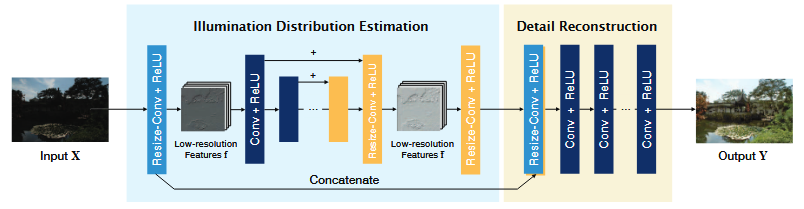
\includegraphics[width=0.8\columnwidth]{GLADNet}
				
				\begin{subfigure}{0.25\textwidth}
					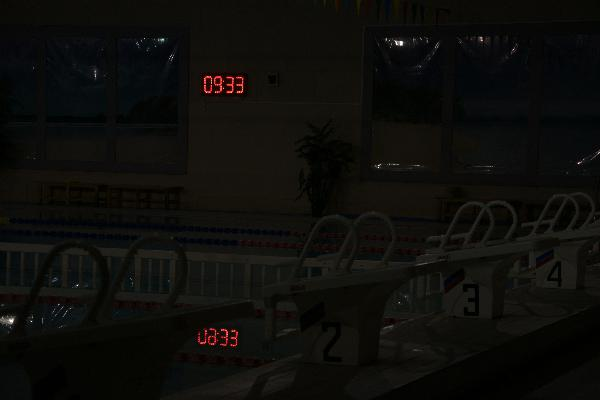
\includegraphics[width=\linewidth]{picture/Input}
					\captionsetup{font=scriptsize}
					\caption{Input}
					\label{fig: Input}
				\end{subfigure}
				\begin{subfigure}{0.25\textwidth}
					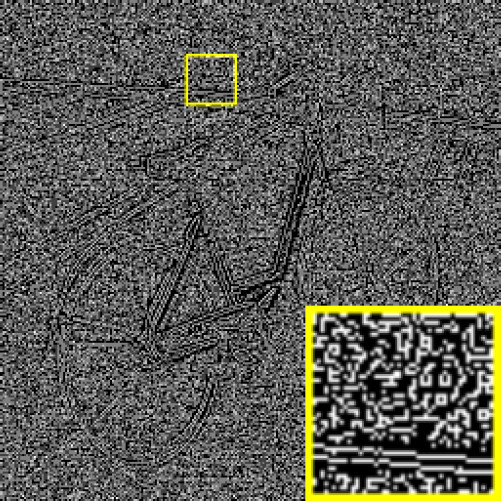
\includegraphics[width=\linewidth]{picture/Structure of (a)}
					\captionsetup{font=scriptsize}
					\caption{Structure of (a)}
					\label{fig: Structure of (a)}
				\end{subfigure}
				\begin{subfigure}{0.25\textwidth}
					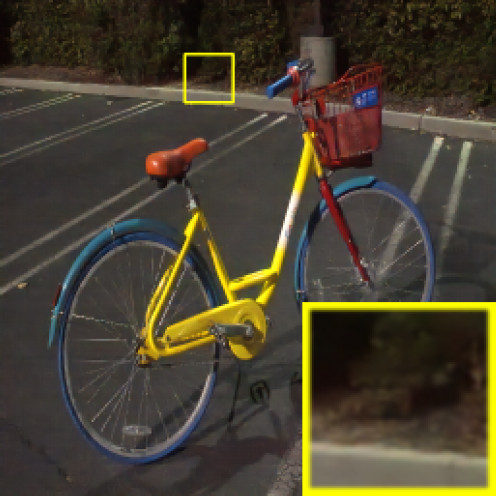
\includegraphics[width=\linewidth]{picture/SNR (CVPR 2022)}
					\captionsetup{font=scriptsize}
					\caption{SNR (CVPR 2022)}
					\label{fig: SNR (CVPR 2022)}	
				\end{subfigure} \\
				\begin{subfigure}{0.25\textwidth}
					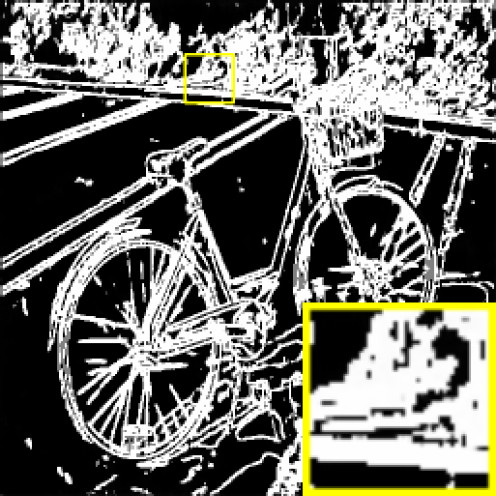
\includegraphics[width=\linewidth]{picture/Structure Modeling}
					\captionsetup{font=scriptsize}
					\caption{Structure Modeling}
					\label{fig: Structure Modeling}
				\end{subfigure}
				\begin{subfigure}{0.25\textwidth}
					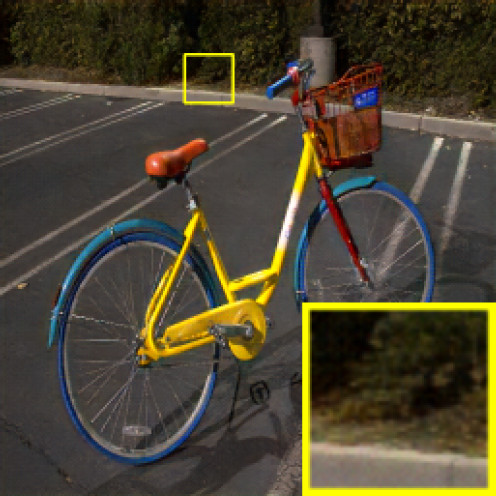
\includegraphics[width=\linewidth]{picture/Ours}
					\captionsetup{font=scriptsize}
					\caption{Ours}
					\label{fig: Ours}
				\end{subfigure}
				\begin{subfigure}{0.25\textwidth}
					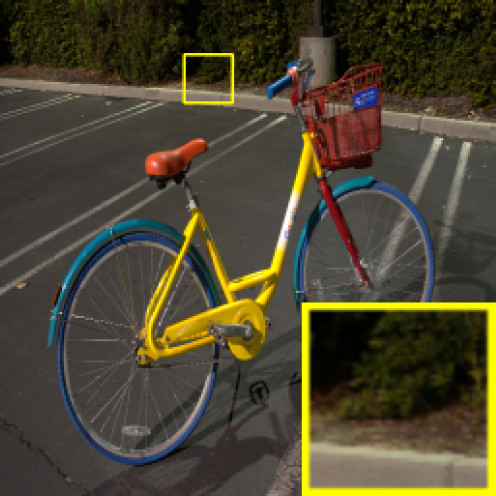
\includegraphics[width=\linewidth]{picture/Ground Truth}
					\captionsetup{font=scriptsize}
					\caption{Ground Truth}
					\label{fig: Ground Truth}
				\end{subfigure}
				
				\captionsetup{font=scriptsize}
				\caption{
					\label{fig: Structural Information}
					A challenging low-light frame (a), from SID-sRGB\cite{chen2018learning},
					enhanced by a SOTA method (c) and our method (e). Our method
					can synthesize the structure map (d) from the input image, leading
					to clearer details, more distinct contrast, and more vivid color. Although
					(c) has high PSNR as 28.17, its SSIM is low as 0.75. Ours
					achieves high scores for both dB and SSIM, as 28.60dB and 0.80.
				}
			\end{figure}
			
			论文提出了一种基于GAN Loss的模型去对结构信息建模,通过获得的结构信息指导增强。如Fig. \ref{fig: Structural Information},低光照图片中很难提取到好的结构信息,论文中提出的方法提取到的结构信息会好很多,并且用于指导图像增强也取得更好的效果。
			
			\subsubsection{Approach}
			
			\begin{itemize}
				\item [(1)]
				首先,通过一个简单的 U-Net 去对外观建模,可以理解成先简单地学习到一个正常光照的 coarse version。其中,损失函数为一个重建损失加感知损失。
				\item [(2)]
				对于结构信息建模部分,借鉴了GAN prior \cite{4767851}的思路,但是不用预训练的 GAN 模型。这里设计到一个结构特征的提取 Structure-Aware Feature Extractor (SAFE)\footnote{SAFE 通过空间变化的操作从黑暗图像及其梯度中提取结构感知的特征(采用自适应的长期和短程计算),提取的结构感知张量输入解码器部分以生成所需的结构映射。。} 
				\item [(3)]
				为了利用得到的结构图来提高外观,本文设计了一个结构导向增强模块 Structure-Guided Enhancement Module(SGEM模块) 初始外观建模结果。在 SGEM 中,根据结构映射生成空间自适应核和归一化参数。然后,对 SGEM 解码器的每一层的特征进行空间全处理$y-$自适应卷积和归一化。虽然 SGEM 的整体架构采用了一个简单的 U-Net 的形式,但它可以有效地增强原始的外观。
			\end{itemize}
			
			\subsubsection{Future}
			-
			
		\subsection{You Do Not Need Additional Priors or Regularizers in Retinex-Based Low-Light Image Enhancement}
		\paragraph{(CVPR 2023)} [未提供数据集]
			
			\subsubsection{Research Background}
			
			之前的工作通过引入一些额外的先验或正则化器来解决低光照增强,但这些手工设计良好的正则化函数很难应用于所有函数,约束过多的联合优化也导致了自适应性和效率的缺失。因此,以前的基于 Retinex 的方法经常会产生非自然的图像。
			
			\subsubsection{Contribution}
			
			\begin{itemize}
				\item [(1)]
				本文提出了一种对比学习方法和一种自知识蒸馏的方法用于 Retinex 分解。
				\item [(2)]
				引入了一种新的对比学习损失函数,其中考虑了一些低质量的负样本。
				\item [(3)]
				在此基础上,提出了一种自我知识提炼的渐进式学习策略,使学生能够更有效地学习教师的知识。
			\end{itemize}

			\subsubsection{Approach}
			
			\begin{itemize}
				\item [(1)]
				本文提出的 Regularizer-free 的 Retinex 分解和合成网络 (RFR) 可以在没有额外的先验或正则化器的情况下进行训练。作者认为手工设计的 Retinex 先验总归不太准确,因此要抛弃手工设计的先验,所以缩减了目标函数。但是,如果使用缩减的 Retinex 公式直接训练,会导致 R 分量的估计可能无效,因为只要对所有的图片都预测一个相同的 R 分量即可。为此引入对比学习\footnote{对比学习 (Contrastive learning) 是一种无监督学习方法,它通过比较不同数据之间的相似性和差异性来学习数据的表示。其中,模型被训练来区分来自同一类别的数据和来自不同类别的数据,从而学习到能够区分不同类别的数据表示。以上,对比学习被用来监督 R 分量的估计,以确保模型能够对不同图像预测出不同的 R 分量。}来监督 R 分量的估计\footnote{具体过程:对一张输入的暗图 $I_{l_i}$},其对应的亮图 $I_{n_i}$ 作为 positive sample,不对应的亮图 $I_{n_k}$ 作为 negative sample。同时,为了避免数据集上可能出现相同或者相似场景, $I_{n_k}$ 和 $I_{n_i}$ 之间的 $ \text{SSIM}_{\omega_{i,k}}$ 来进行归一化。
				\item [(2)]
				作为对对比学习的补充,文章还提出了另一种训练方式(独立于前面的对比学习,也就是说要么用对比学习要么用自蒸馏学习)。利用亮图的R分量估计特征来蒸馏暗图的 R 分量估计特征(其实如果用的是同一个网络的话是可以不看做自蒸馏的,但是文章用的是两个相同结构不同参数的网络,一个作为教师网络学习亮图的 R 分量估计特征,一个作为学生网络学习暗图的 R 分量估计特征,这就和蒸馏学习的流程一摸一样了)\footnote{自蒸馏学习 (Self-distillation) 和蒸馏学习 (Distillation learning) 都是一种用于模型压缩的方法,它们通过将一个大型模型的知识迁移到一个小型模型中来实现模型压缩。
					
				蒸馏学习通常指使用一个大型的教师模型来指导一个小型的学生模型的训练。在这种方法中,教师模型首先被训练好,然后它的输出被用作学生模型的训练目标。通过这种方式,学生模型能够从教师模型中学习到知识,从而达到压缩模型的目的。
				
				自蒸馏学习则是一种特殊的蒸馏学习方法,它不需要额外的教师模型,而是直接使用学生模型自身作为教师。在这种方法中,学生模型首先被训练好,然后它自身的输出被用作训练目标。通过这种方式,学生模型能够从自身中学习到知识,从而达到压缩模型的目的。}
				
			\end{itemize}
			
			\subsubsection{Future}
			
			本文利用自蒸馏和对比学习来提供额外监督是个很不错的方法,文章根据暗图增强任务进行了适应性的调整,取得的效果也很好,实验充分。后续可以把这类的方法应用到监督学习方法中。
		
%	\begin{table}[!htbp]
%		\centering
%		\small
%		\caption{\label{tab: Datasets comparison}
%			Comparison between classic LLIE datasets
%			and our UHD-LL dataset. ‘Number’: the number of
%			paired images. ‘Resolution’: the average resolution of the
%			dataset. ‘Noise’: low-light images contain noise. ‘Real’:
%			both low-light images and GT are acquired in real scenes.} %表格的标题
%		%\resizebox{\textwidth}{!}{ %按照宽度调整调整表格大小
%			\begin{tabular}{>{\centering\arraybackslash}m{2.6cm}|c|c|c|c}
%				
%				\hline
%				
%				\textbf{Dataset} & \textbf{Number} & \textbf{Resolution} & \textbf{Noise} & \textbf{Real} \\
%				
%				\hline
%				
%				SID(RAW) & 5094 & \makecell{4240 $\times$ 2832 \\ 6000 $\times$ 4000} & \checkmark & \checkmark \\ 
%				MIT-Adobe FiveK & 5000 & 4000 $\times$ 2500 &  &  \\ 
%				Exposure-Errors  & 24000 & 1000 $\times$ 900 &  &  \\
%				LOL & 500/789 & 600 $\times$ 400 & \checkmark & \checkmark \\
%				\textbf{UHD-LL(Ours)} & \textbf{2150} & \textbf{3840 $\times$ 2160} & \checkmark & \checkmark \\
%				
%				\hline
%				
%			\end{tabular}
%			%}
%		\captionsetup{font=scriptsize} %设置标题字体与表格字体一致
%	\end{table}
	
	\part{Unity VR 开发计划}
	
		\section{环境配置}

		\begin{itemize}
			\item [(1)] 
			Unity 2019.4.28f1c1 及以上版本。
			
			\item [(2)]
			采用 Unity 3D 引擎,采用 Open XR 和 Steam VR 拓展包\footnote{Unity 3D 支持创建 3D 和 2D 游戏以及其他交互式内容。Unity VR 则是 Unity 3D 的一个扩展,它支持开发虚拟现实(VR)应用程序。Unity VR 提供了一系列工具和功能,可以帮助开发人员创建沉浸式的 VR 体验。}。
		\end{itemize}

		\section{开发计划}
	
			\subsection{模拟海洋水系统}
	
			构建海洋水系统,该水系统可有模拟波浪和泡沫效果,可以实现水体运动,模拟浮力,且需能够同时渲染多个摄像机(VR 开发)。同时,该水系统可以模拟光传输,包括反射、折射、散射、焦散近似、阴影。此外,光散射和波浪衰减也需要实现。
		
			\begin{itemize}
				\item [(1)] 
				在 Unity VR 开发中,使用 Shader Graph 和 Particle System 等工具来构建一个具有不同天气和波浪的海洋水系统。一种常用的方法是使用 Unity 的 Shader Graph 来创建一个动态的海洋水面材质,在 Shader Graph 中定义不同的参数,例如波浪高度、波浪速度和波浪方向等,然后使用脚本来动态控制这些参数,以实现不同天气下海洋水面的变化。
			
				\item [(2)]
				Unity 商店中有许多现成的插件和资源包,可以帮助快速实现海洋水系统。但存在一个很大的问题,\textcolor{red}{很多 packages 不支持同时渲染多个摄像机,这说明这些包往往不适配 VR 项目,因此需要对这些 Package中的 Assets 进行移植。} 所以,这里关注的重点可以在如何移植上,或如何让该包支持渲染多摄像机。如 Crest 实现了上述绝大部分的功能,但是不支持同时渲染多个摄像机。此外,很多海洋水系统资源包对于高级水模拟项目,并不能简单的即插即用,需要技术设置和配置\footnote{Crest 是一个功能丰富的海洋,针对 PC 和游戏机平台 以及 Unity 2019.4.8 及以上版本}。
				
				\item [(3)]
				完成上述两个步骤之后,后续的开发目标为增加更多风浪和船只航行状态,提高模拟器的真实性和准确性。
			\end{itemize}
	
			\subsection{船只模型}
		
			可以考虑使用原来项目的船只模型。
	
	

	%	\section{Analysis}
	
	%	In this section you will need to show your experimental results. Use tables and
	%	graphs when it is possible. Table~\ref{tbl:bins} is an example.
	
	%	\begin{table}[ht]
		%		\begin{center}
			%			\caption{Every table needs a caption.}
			%			\label{tbl:bins} % spaces are big no-no withing labels
			%			\begin{tabular}{|ccc|} 
				%				\hline
				%				\multicolumn{1}{|c}{$x$ (m)} & \multicolumn{1}{c|}{$V$ (V)} & \multicolumn{1}{c|}{$V$ (V)} \\
				%				\hline
				%				0.0044151 &   0.0030871 &   0.0030871\\
				%				0.0021633 &   0.0021343 &   0.0030871\\
				%				0.0003600 &   0.0018642 &   0.0030871\\
				%				0.0023831 &   0.0013287 &   0.0030871\\
				%				\hline
				%			\end{tabular}
			%		\end{center}
		%	\end{table}
	%	
	%	Analysis of equation~\ref{eq:aperp} shows ...
	%	
	%	Note: this section can be integrated with the previous one as long as you
	%	address the issue. Here explain how you determine uncertainties for different
	%	measured values. Suppose that in the experiment you make a series of
	%	measurements of a resistance of the wire $R$ for different applied voltages
	%	$V$, then you calculate the temperature from the resistance using a known
	%	equation and make a plot  temperature vs. voltage squared. Again suppose that
	%	this dependence is expected to be linear~\cite{Cyr}, and the proportionality coefficient
	%	is extracted from the graph. Then what you need to explain is that for the
	%	resistance and the voltage the uncertainties are instrumental (since each
	%	measurements in done only once), and they are $\dots$. Then give an equation
	%	for calculating the uncertainty of the temperature from the resistance
	%	uncertainty. Finally explain how the uncertainty of the slop of the graph was
	%	found (computer fitting, graphical method, \emph{etc}.)
	%	
	%	If in the process of data analysis you found any noticeable systematic
	%	error(s), you have to explain them in this section of the report.
	%	
	%	It is also recommended to plot the data graphically to efficiently illustrate
	%	any points of discussion. For example, it is easy to conclude that the
	%	experiment and theory match each other rather well if you look at
	%	Fig.~\ref{fig:samplesetup} and Fig.~\ref{fig:exp_plots}.
	%	
	%	\begin{figure}[ht] 
		%		\centering
		%		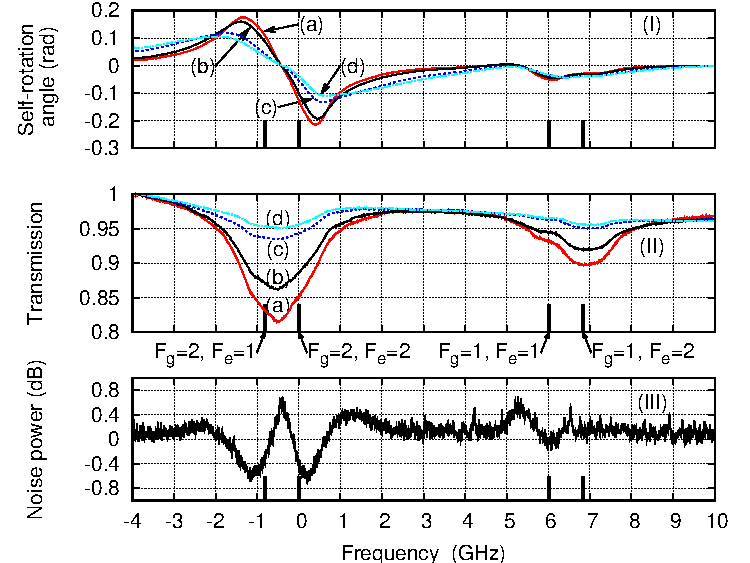
\includegraphics[width=0.5\columnwidth]{sr_squeezing_vs_detuning}
		%		
		%		% some figures do not need to be too wide
		%		\caption{
			%			\label{fig:exp_plots}  
			%			Every plot must have axes labeled.
			%		}
		%	\end{figure}
	
	
	%	\section{Conclusions}
	%	Here you briefly summarize your findings.
	
	%++++++++++++++++++++++++++++++++++++++++
	% References section will be created automatically 
	% with inclusion of "thebibliography" environment
	% as it shown below. See text starting with line
	% \begin{thebibliography}{99}
		% Note: with this approach it is YOUR responsibility to put them in order
		% of appearance.
		
		\renewcommand{\refname}{References}
		
		
		%	\begin{thebibliography}{00}
			
			%		\bibitem{b1}\label{cite:b1}
			%		W. Wang, C. Wei, W. Yang and J. Liu, "GLADNet: Low-Light Enhancement Network with Global Awareness," 2018 13th IEEE International Conference on Automatic Face \& Gesture Recognition (FG 2018), Xi'an, China, 2018, pp. 751-755, DOI: 10.1109/FG.2018.00118.
			
			%		\bibitem{b2}\label{cite:b2}
			%		A.\ Mahajan, K.\ Somaraj and M. Sameer, "Adopting Artificial Intelligence Powered ConvNet To Detect Epileptic Seizures," 2020 IEEE-EMBS Conference on Biomedical Engineering and Sciences (IECBES), Langkawi Island, Malaysia, 2021, pp. 427-432, DOI: 10.1109/IECBES48179.2021.9398832.
			
			%		\bibitem{Cyr}
			%		N.\ Cyr, M.\ T$\hat{e}$tu, and M.\ Breton,
			% "All-optical microwave frequency standard: a proposal,"
			%		IEEE Trans.\ Instrum.\ Meas.\ \textbf{42}, 640 (1993).
			
			
			
			%	\end{thebibliography}
		
		\bibliographystyle{unsrt}
		\bibliography{reference}
		
		
	\end{document}
